%%%%%%%%%%%%%%%%%%%%%%%%%%%%%%%%%%%%%%%%%%%%%%%%%%%%%%%%%%%%%
%% HEADER
%%%%%%%%%%%%%%%%%%%%%%%%%%%%%%%%%%%%%%%%%%%%%%%%%%%%%%%%%%%%%
%%
%%
\newcommand{\hyperrefpdfauthor}{}
\newcommand{\hyperrefpdftitle}{}
\newcommand{\hyperrefpdfsubject}{}
\newcommand{\hyperrefpdfkeywords}{}
\newcommand{\hyperrefpdfborder}{0}
\documentclass[master]{wissdoc-kw-eng} % possible options: bachelor, master, diploma, phdsubmitted (vorgelegte Dissertation), phdapproved (genehmigte Dissertation)
% additional logo options: fkie (for Fraunhofer FKIE logo on the left), iop (to use a combiend COMSYS and Internet of Production logo on the right)

\usepackage{pdfpages}

\usepackage{acro}

\makeatletter
\@ifpackagelater{acro}{2017/02/17}{\@ifpackagelater{acro}{2019/09/23}{}{
	\let\IDeclareAcronym\DeclareAcronym
	\renewcommand{\DeclareAcronym}[2]{%
		\IDeclareAcronym{#1}{%
		#2,foreign-plural={}
		}
	}
}}{}
\makeatother

\newcommand\ifacrothree{%
	\ifnum\numexpr\csname c_acro_version_major_number_tl\endcsname=3\relax
}

\ifacrothree
	\acsetup{use-id-as-short}
	\def\ProvideAcroEnding{\DeclareAcroEnding}
\fi

\ProvideAcroEnding{possessive}{'s}{'s}
\ProvideAcroEnding{possessiveplural}{s'}{s'}

\ifacrothree
	\NewAcroCommand\acg{m}{%
		\acropossessive
		\UseAcroTemplate{first}{#1}%
	}
	\NewAcroCommand\acsg{m}{%
		\acropossessive
		\UseAcroTemplate{short}{#1}%
	}
	\NewAcroCommand\aclg{m}{%
		\acropossessive
		\UseAcroTemplate{long}{#1}%
	}
	\NewAcroCommand\acgp{m}{%
		\acropossessiveplural
		\UseAcroTemplate{first}{#1}%
	}
	\NewAcroCommand\acsgp{m}{%
		\acropossessiveplural
		\UseAcroTemplate{short}{#1}%
	}
	\NewAcroCommand\aclgp{m}{%
		\acropossessiveplural
		\UseAcroTemplate{long}{#1}%
	}
\else
	% remove this part when acro-2 (texlive-2019) is no longer in use by any sane person
	% e.g. ubuntu-20.04 has texlive-2019 and will receive updates until April 2025
	\ExplSyntaxOn
	\NewAcroCommand \acg {
		\acro_possessive:
		\acro_use:n {#1}
	}
	\NewAcroCommand \acsg {
		\acro_possessive:
		\acro_short:n {#1}
	}
	\NewAcroCommand \aclg {
		\acro_possessive:
		\acro_long:n {#1}
	}
	\NewAcroCommand \acgp {
		\acro_possessiveplural:
		\acro_use:n {#1}
	}
	\NewAcroCommand \acsgp {
		\acro_possessiveplural:
		\acro_short:n {#1}
	}
	\NewAcroCommand \aclgp {
		\acro_possessiveplural:
		\acro_long:n {#1}
	}
	\ExplSyntaxOff
\fi

% By default, LaTeX uses the acronym name as its short form
\DeclareAcronym{LP}{short=LP,long=Logical Process,short-indefinite=an,long-plural=es}
% You should explicitly set the short form (e.g., if you want lowercase acronym names) to avoid a warning,
% in this case you MUST specify the short= keyword as the first one.
% Otherwise, the document doesen't currently compile under MacTeX (at least).
\DeclareAcronym{abc}{short=ABC,long=Alphabet,short-indefinite=an,long-indefinite=an}



\usepackage{multibib}
\newcites{own}{Pre-published Papers}

% % newer acronym packaged dont use bflabel anymore,
\providecommand\aclabelfont{} % the new command ist aclabelfont however, we also need to be backwards compatible so... we do it like this
\renewcommand{\aclabelfont}[1]{\normalfont{\normalsize{#1}}\hfill} % keine serifenlose schrift für acronym

% newer acronym packaged dont use bflabel anymore, to not fail the statement below provide the command if not existing
\providecommand\bflabel{}
\renewcommand{\bflabel}[1]{\aclabelfont{#1}}

\usepackage{float}
\floatstyle{ruled}
\newfloat{listing}{htbp}{lop}[chapter]
\floatname{listing}{Listing}

%% zur Zitaten des Quelltextes%%%%%%%%%%%%%%%%%%%%%%%%%%%%%%%
% "final" forces printing of all listings, even if the global "draft" is set
\usepackage[final]{listings}
\lstset{
    language=C++,
    basicstyle=\footnotesize\ttfamily,
    tabsize=2,
    numberstyle=\tiny\color{gray},
    numbersep=5pt,
    numbers=left,
    captionpos=b,
    abovecaptionskip=0pt,
    belowcaptionskip=0pt,
    aboveskip=10pt,
    belowskip=0pt,
    floatplacement=tbp,
    frame=topline,
    framerule=.1pt,
    framesep = 3pt,
    mathescape=true,
    boxpos=t,
    xleftmargin=1.2em,
}

\renewcommand\lstlistingname{\textbf{Listing}}
% This is only kept for backwards compatibility. You should never have to use it. Use the listing-environment instead.
%\DeclareCaptionFormat*{lstruled}{{\bfseries#1\small\space\normalfont#3\hrule height.1pt depth0pt}\par}
%\captionsetup[lstlisting]{format=lstruled,singlelinecheck=false}

%% Stil der Beschriftungen %%%%%%%%%%%%%%%%%%%%%%%%%%%%%%%%%%
\usepackage{caption}
\captionsetup[figure]{font={small,sf}}
\captionsetup[subfigure]{justification=centering,font={small,sf}}
\captionsetup[table]{font={small,sf}}
\captionsetup[listing]{font={small,sf}}

%% Normales LaTeX oder pdfLaTeX? %%%%%%%%%%%%%%%%%%%%%%%%%%%%
%% ==> Das neue if-Kommando "\ifpdf" wird an einigen wenigen
%% ==> Stellen benötigt, um die Kompatibilität zwischen
%% ==> LaTeX und pdfLaTeX herzustellen.
%\newif\ifpdf
%\ifx\pdfoutput\undefined
%    \pdffalse              %%normales LaTeX wird ausgeführt
%\else
%    \pdfoutput=1
%    \pdftrue               %%pdfLaTeX wird ausgeführt
%\fi

%% Deutsche Anpassungen %%%%%%%%%%%%%%%%%%%%%%%%%%%%%%%%%%%%%
\usepackage[T1]{fontenc}
\usepackage[utf8]{inputenc}

%% mehrere Abbildungen in eine %%%%%%%%%%%%%%%%%%%%%%%%%%%%%%
\usepackage{subcaption}

%% Packages für Formeln %%%%%%%%%%%%%%%%%%%%%%%%%%%%%%%%%%%%%
\usepackage{amsmath}
\usepackage{amsfonts}

\usepackage[inline]{enumitem}
\setlist[description]{font=\sffamily\bfseries}
\usepackage[capitalise,nameinlink,noabbrev]{cleveref}

%% Zeilenabstand %%%%%%%%%%%%%%%%%%%%%%%%%%%%%%%%%%%%%%%%%%%%
\usepackage{setspace}
%\singlespacing        %% 1-zeilig (Standard)
%\onehalfspacing       %% 1,5-zeilig
%\doublespacing        %% 2-zeilig

%% Andere Packages %%%%%%%%%%%%%%%%%%%%%%%%%%%%%%%%%%%%%%%%%%
%\usepackage{a4wide} %%Kleinere Seitenränder = mehr Text pro Zeile.
\usepackage{fancyhdr} %%Fancy Kopf- und Fußzeilen
%\usepackage{longtable} %%Für Tabellen, die eine Seite überschreiten
\usepackage{lscape}
\usepackage{rotating}
%\usepackage[htt]{hyphenat} %Trennung von Typewriter-Schriften
%\usepackage{listings}
\usepackage{tikz}
\usetikzlibrary{calc}
\usepackage[en-US]{datetime2} %%Automatisches Ausfüllen der eidesstattlichen Versicherung

% Tabellen mit Center und left
\usepackage{tabularx,colortbl} % colored table background
\newcolumntype{C}[1]{>{\centering\arraybackslash}p{#1}}
\newcolumntype{R}[1]{>{\raggedleft\arraybackslash}p{#1}}
% Table spacings
\newcommand\T{\rule{0pt}{2.5ex}\rule[-1.0ex]{0pt}{0pt}}
\newcommand\B{\rule[-1.0ex]{0pt}{0pt}}

\definecolor{slightgray}{gray}{.90}


% Put your own defs to definitions.tex, so you don't need to fiddle around with this file.
\IfFileExists{definitions.tex}{\input{definitions.tex}}{}

%% zur Benutzung bei ergänzenden Daten%%%%%%%%%%%%%%%%%%%%%%%%
%\usepackage{endnotes}
%\renewcommand{\notesname}{Konfigurationsdaten der Messreihen}
%\renewcommand{\theendnote}{\Alph{endnote}}
%\renewcommand{\enotesize}{\normalsize}

%\hyphenation{Sensor-netz-werk
%}

%%%%%%%%%%%%%%%%%%%%%%%%%%%%%%%%%%%%%%%%%%%%%%%%%%%%%%%%%%%%%
%% DOKUMENT
%%%%%%%%%%%%%%%%%%%%%%%%%%%%%%%%%%%%%%%%%%%%%%%%%%%%%%%%%%%%%

% Use the following for selectively updating only individual
% chapters. Multiple chapters can be included as a comma-separated
% list.

% \includeonly{chapters/00_introduction.tex}

\begin{document}

%% Dateiendungen für Grafiken %%%%%%%%%%%%%%%%%%%%%%%%%%%%%%%
%% ==> Sie können hiermit die Dateiendung einer Grafik weglassen.
%% ==> Aus "\includegraphics{titel.eps}" wird "\includegraphics{titel}".
%% ==> Wenn Sie nunmehr 2 inhaltsgleiche Grafiken "titel.eps" und
%% ==> "titel.pdf" erstellen, wird jeweils nur die Grafik eingebunden,
%% ==> die von ihrem Compiler verarbeitet werden kann.
%% ==> pdfLaTeX benutzt "titel.pdf". LaTeX benutzt "titel.eps".
%\ifpdf
%    \DeclareGraphicsExtensions{.pdf,.jpg,.png}
%\else
%    \DeclareGraphicsExtensions{.eps}
%\fi

\pagestyle{empty} %%Keine Kopf-/Fusszeilen auf den ersten Seiten.

\ifnotdraft{
%% Deckblatt %%%%%%%%%%%%%%%%%%%%%%%%%%%%%%%%%%%%%%%%%%%%%%%%
\frontmatter
% !TEX root = ../thesis.tex

\newcommand{\thesistitleA}{% Note the %-symbol at end of the line of each command
Your Awesome Thesis Title%
}
\newcommand{\thesistitleB}{%
(Which May Also Be Quite Long%
}
\newcommand{\thesistitleC}{%
And Stretch Several Lines) Here%
}
\newcommand{\firstname}{%
Your Firstname(s)%
}
\newcommand{\lastname}{%
Your Lastname(s)%
}
\newcommand{\studentid}{%
XXX XXX % This is optional, remove text if you do not want to specific your student id
}
\newcommand{\currentdegree}{%
Master of Science % only for PhD thesis, typically your current degree is Master of Science if you're writing your PhD thesis
}
\newcommand{\aimeddegreeGermanPossesive}{% only for PhD thesis. Degree you are about to get in German, possesive case, including indefinite article
% reasonable options: eines Doktors der Naturwissenschaften, einer Doktorin der Naturwissenschaften, eines Doktors der Ingenieurwissenschaften, einer Doktorin der Ingenieurwissenschaften
eines Doktors der Naturwissenschaften%
}
\newcommand{\placeofbirth}{%
Your Place of Birth % only for PhD thesis, include land if land!=Germany
}
\DTMsavedate{RegistrationDate}{2019-01-01} % only undergrad
\DTMsavedate{SubmissionDate}{2019-08-30} % undergrad and phd
\DTMsavedate{DefenseDate}{2019-08-30} % only phdapproved

\newcommand{\advisers}{% only undergrad
Dipl.-Inform. Erika Mustermann\\
Max Mustermann, M.$\,$Sc.%
}
\newcommand{\examiners}{%
Prof.~Dr.-Ing. Klaus Wehrle\\
Prof.~Dr.~rer.nat. Albert Einstein%
}



% Usually, you do NOT have to change information below.

\begin{titlepage}
\pdfbookmark[0]{Title Page}{Title Page}

% for PhD theses this needs to conform with the chair regulations (Promotions-Merkblatt komplett, Homepage Promotionsbuero Fakultät 1, RWTH Aachen)!

\ifundergrad
	\ifiop
		\tikz[overlay,remember picture]\node[inner sep=0,anchor=north east] at ($(current page.north east)+(2cm,1.7cm)$) {%
			
\includegraphics[width=15cm,keepaspectratio]{logos/comsys-iop-rwth}%
		};
	\else
		\tikz[overlay,remember picture]\node[inner sep=0,anchor=north east] at ($(current page.north east)+(2.5cm,2.5cm)$) {%
			
\includegraphics[height=3.2cm,keepaspectratio]{logos/rwth_comsys_bild_cmyk}%
		};
	\fi
	\iffkie
		\tikz[overlay,remember picture]\node[inner sep=0,anchor=north west] at ($(current page.north west)+(4cm,1.7cm)$) {%
			
\includegraphics[width=6cm,keepaspectratio]{logos/fkie_60mm_p334}%
		};
	\fi
\fi

\hbox{}
\vfill % vertically center text on page

\centering

\ifundergrad
	\def\titleformat{\huge\sffamily}
\fi
\ifphd
	\def\titleformat{\LARGE}
\fi

{\titleformat\textbf{%
\phantom{g}\thesistitleA\phantom{g}\\[.1em]
\phantom{g}\thesistitleB\phantom{g}\\[.1em]
\phantom{g}\thesistitleC\phantom{g}\\[.1em]
}}

\vskip 2cm

\ifundergrad
{\large\sffamily

\ifbachelor Bachelor \fi\ifmaster Master \fi\ifdiploma Diploma \fi Thesis\\[5pt]
\textbf{\firstname{} \lastname{}}
\vskip 1cm

The present work was submitted to the\\[5pt]
\textbf{Chair of Communication and Distributed Systems\\[5pt]
        RWTH Aachen University, Germany}
\vskip 2cm

Advisor(s):
\vskip 2mm
\advisers{}
\vskip 5mm
Examiners:
\vskip 2mm
\examiners{}
\vskip 1cm

\begin{tabular}{R{6cm}p{6cm}}
Registration date:  & \DTMusedate{RegistrationDate} \\
Submission date:    & \DTMusedate{SubmissionDate} \\
\end{tabular}

} %\large\sffamily
\fi

\ifphd
\ifphdsubmitted
Der Fakult\"at f\"ur Mathematik, Informatik und Naturwissenschaften\\der RWTH Aachen University vorgelegte Dissertation zur Erlangung\\des akademischen Grades \aimeddegreeGermanPossesive{}
\fi
\ifphdapproved
Von der Fakult\"at f\"ur Mathematik, Informatik und Naturwissenschaften\\der RWTH Aachen University zur Erlangung des akademischen Grades\\\aimeddegreeGermanPossesive{} genehmigte Dissertation
\fi

\vspace{2cm}
\ifphdsubmitted
von
\fi
\ifphdapproved
vorgelegt von
\fi

\vspace{2cm}
\currentdegree{}\\
\vspace{1em}
{\large{\textbf{\firstname{} \lastname{}}}}\\
\vspace{1em}
aus \placeofbirth{}

\ifphdsubmitted
\vspace{7cm}
\fi

\ifphdapproved
\vspace{2cm}
Berichter:\\
\vspace{1em}
\examiners{}\\
\vspace{2cm}
Tag der m\"undlichen Pr\"ufung: {\DTMsetup{datesep=.}\DTMsetstyle{ddmmyyyy}\DTMusedate{DefenseDate}}
\fi
\fi

\vfill % vertically center text on page

\end{titlepage}


\cleardoublepage
\ifundergrad
% !TEX root = ../thesis.tex

\ifbachelor
\includepdf[pages={1},offset=75 -75,pagecommand={
\begin{tikzpicture}[remember picture,overlay,shift={(current page.center)}]
\coordinate (de_begin-de_generic) at (5.4,10.3);
\coordinate (de_end-de_generic) at (6.4,10.3);
\coordinate (de_begin-de_master) at (-5.35,9.8);
\coordinate (de_end-de_master) at (-3.2,9.8);
\coordinate (en_begin-en_generic) at (3.2,9.35);
\coordinate (en_end-en_generic) at (3.9,9.35);
\coordinate (en_begin-en_master) at (6.0,9.35);
\coordinate (en_end-en_master) at (7.65,9.35);
\node at (-5.5,12.1)
       [text width=7cm,rounded corners,below right]
{
\mbox{\lastname{}, \firstname{}}
};
\node at (3.25,12.1)
       [text width=5cm,rounded corners,below right]
{
\studentid{}
};
\draw[line width=1mm] (de_begin-de_generic) -- (de_end-de_generic);
\draw[line width=1mm] (de_begin-de_master) -- (de_end-de_master);
\draw[line width=0.5mm] (en_begin-en_generic) -- (en_end-en_generic);
\draw[line width=0.5mm] (en_begin-en_master) -- (en_end-en_master);
\node at (-5.5,8.95)
       [text width=16.5cm,rounded corners,below right]
{
\begin{onehalfspacing}%
\thesistitleA\phantom{g}\\[0.1em]
\thesistitleB\phantom{g}\\[0.1em]
\thesistitleC\phantom{g}\\[0.1em]
\end{onehalfspacing}
};
\node at (-5.5,2.35)
       [text width=7cm,rounded corners,below right]
{
Aachen, {\DTMsetup{datesep=.}\DTMsetstyle{ddmmyyyy}\DTMusedate{SubmissionDate}}
};
\node at (-5.5,-8.7)
       [text width=7cm,rounded corners,below right]
{
Aachen, {\DTMsetup{datesep=.}\DTMsetstyle{ddmmyyyy}\DTMusedate{SubmissionDate}}
};
\end{tikzpicture}
}]{Formular_Eidesstattliche_Versicherung_neu.pdf}
\fi

\ifmaster
\includepdf[pages={1},offset=75 -75,pagecommand={
\begin{tikzpicture}[remember picture,overlay,shift={(current page.center)}]
\coordinate (de_begin-de_generic) at (5.4,10.3);
\coordinate (de_end-de_generic) at (6.4,10.3);
\coordinate (de_begin-de_bachelor) at (6.5,10.3);
\coordinate (de_end-de_bachelor) at (9,10.3);
\coordinate (en_begin-en_generic) at (3.2,9.35);
\coordinate (en_end-en_generic) at (3.9,9.35);
\coordinate (en_begin-en_bachelor) at (4.0,9.35);
\coordinate (en_end-en_bachelor) at (5.9,9.35);
\node at (-5.5,12.1)
       [text width=7cm,rounded corners,below right]
{
\mbox{\lastname{}, \firstname{}}
};
\node at (3.25,12.1)
       [text width=5cm,rounded corners,below right]
{
\studentid{}
};
\draw[line width=1mm] (de_begin-de_generic) -- (de_end-de_generic);
\draw[line width=1mm] (de_begin-de_bachelor) -- (de_end-de_bachelor);
\draw[line width=0.5mm] (en_begin-en_generic) -- (en_end-en_generic);
\draw[line width=0.5mm] (en_begin-en_bachelor) -- (en_end-en_bachelor);
\node at (-5.5,8.95)
       [text width=16.5cm,rounded corners,below right]
{
\begin{onehalfspacing}%
\thesistitleA\phantom{g}\\[0.1em]
\thesistitleB\phantom{g}\\[0.1em]
\thesistitleC\phantom{g}\\[0.1em]
\end{onehalfspacing}
};
\node at (-5.5,2.35)
       [text width=7cm,rounded corners,below right]
{
Aachen, {\DTMsetup{datesep=.}\DTMsetstyle{ddmmyyyy}\DTMusedate{SubmissionDate}}
};
\node at (-5.5,-8.7)
       [text width=7cm,rounded corners,below right]
{
Aachen, {\DTMsetup{datesep=.}\DTMsetstyle{ddmmyyyy}\DTMusedate{SubmissionDate}}
};
\end{tikzpicture}
}]{Formular_Eidesstattliche_Versicherung_neu.pdf}
\fi

\ifdiploma
\includepdf[pages={1},offset=75 -75,pagecommand={
\begin{tikzpicture}[remember picture,overlay,shift={(current page.center)}]
\coordinate (de_begin-de_bachelor) at (6.5,10.3);
\coordinate (de_end-de_bachelor) at (9,10.3);
\coordinate (de_begin-de_master) at (-5.35,9.8);
\coordinate (de_end-de_master) at (-3.2,9.8);
\coordinate (en_begin-en_bachelor) at (4.0,9.35);
\coordinate (en_end-en_bachelor) at (5.9,9.35);
\coordinate (en_begin-en_master) at (6.0,9.35);
\coordinate (en_end-en_master) at (7.65,9.35);
\node at (-5.5,12.1)
       [text width=7cm,rounded corners,below right]
{
\mbox{\lastname{},\firstname{}}
};
\node at (3.25,12.1)
       [text width=5cm,rounded corners,below right]
{
\studentid{}
};
\draw[line width=1mm] (de_begin-de_bachelor) -- (de_end-de_bachelor);
\draw[line width=1mm] (de_begin-de_master) -- (de_end-de_master);
\draw[line width=0.5mm] (en_begin-en_bachelor) -- (en_end-en_bachelor);
\draw[line width=0.5mm] (en_begin-en_master) -- (en_end-en_master);
\node at (-5.5,8.95)
       [text width=16.5cm,rounded corners,below right]
{
\begin{onehalfspacing}%
\thesistitleA\phantom{g}\\[0.1em]
\thesistitleB\phantom{g}\\[0.1em]
\thesistitleC\phantom{g}\\[0.1em]
\end{onehalfspacing}
};
\node at (-5.5,2.35)
       [text width=7cm,rounded corners,below right]
{
Aachen, {\DTMsetup{datesep=.}\DTMsetstyle{ddmmyyyy}\DTMusedate{SubmissionDate}}
};
\node at (-5.5,-8.7)
       [text width=7cm,rounded corners,below right]
{
Aachen, {\DTMsetup{datesep=.}\DTMsetstyle{ddmmyyyy}\DTMusedate{SubmissionDate}}
};
\end{tikzpicture}
}]{Formular_Eidesstattliche_Versicherung_neu.pdf}
\fi

\cleardoublepage
\fi
% !TEX root = ../thesis.tex

\pdfbookmark[0]{Abstract}{Abstract}

\begin{center}
\paragraph{Abstract}
\hrulefill
\end{center}
Außerhalb der Umgebung hingegen erfolgt die Trennung des Donaudampfschifffahrtskapitäns nicht korrekt.


\ifphd
\clearpage % PhD thesis abstracts are commonly about a page...
\fi
\ifundergrad
\vspace {2cm} % ... while undergrad thesis abstracts are commonly about half a page
\fi
% !TEX root = ../thesis.tex

\pdfbookmark[0]{Kurzfassung}{Kurzfassung}

\begin{otherlanguage*}{ngerman}
\begin{center}
\paragraph{Kurzfassung}
\hrulefill
\end{center}
In der \texttt{otherlanguage*}-Umgebung erfolgt die Trennung des Donaudampfschifffahrtskapitäns korrekt.


\end{otherlanguage*}

\cleardoublepage
\ifphdapproved
% !TEX root = ../thesis.tex

\pdfbookmark[0]{Acknowledgments}{Acknowledgments}

\chapter*{Acknowledgments}

Don't forget to thank your dog


\cleardoublepage
\fi
\ifphdsubmitted
% !TEX root = ../thesis.tex

\section*{Declaration of Authorship}
\pdfbookmark[0]{Declaration of Authorship}{Declaration of Authorship}

I, \firstname{} \lastname{}

declare that this thesis and the work presented in it are my own and has been generated by me as the result of my own original research.

I do solemnely swear that:

\begin{enumerate}[label=\arabic*.,topsep=0pt]
	\item This work was done wholly or mainly while in candidature for the doctoral degree at this faculty and university;
	\item Where any part of this thesis has previously been submitted for a degree or any other qualification at this university or any other institution, this has been clearly stated;
	\item Where I have consulted the published work of others or myself, this is always clearly attributed;
	\item Where I have quoted from the work of others or myself, the source is always given.
		This thesis is entirely my own work, with the exception of such quotations;
	\item I have acknowledged all major sources of assistance;
	\item Where the thesis is based on work done by myself jointly with others, I have made clear exactly what was done by others and what I have contributed myself;
	\item Parts of this work have been published before.
		A detailed list can be found on the following page.
\end{enumerate}

\vspace{20pt}
{\DTMsetup{datesep=.}\DTMsetstyle{en-US}\DTMusedate{SubmissionDate}}

\newpage
\section*{Published Papers}
\pdfbookmark[0]{Published Papers}{Published Papers}

Parts of this thesis are based on the following peer-reviewed papers that have already been published.
All my collaborators are among my co-authors.
A detailed attribution of contributions can be found in Section~\ref{...} on page~\pageref{...}.

\subsection*{List of Publications}

\nociteown{*}
\begingroup
	\def\chapter*#1{}
	\bibliographyown{literature/own}
	\bibliographystyleown{styles/comsys-alpha}
\endgroup


\cleardoublepage
\fi

% Titelseite hatte noch normale Tabellen. Von hier ab sollen alle
% Tabellen laut style-Vorgaben sans serif sein.
\AtBeginEnvironment{tabular}{\sffamily}
\AtBeginEnvironment{tabularx}{\sffamily}

%% Inhaltsverzeichnis %%%%%%%%%%%%%%%%%%%%%%%%%%%%%%%%%%%%%%%
\setcounter{tocdepth}{2}
\tableofcontents %Inhaltsverzeichnis
\cleardoublepage %Das erste Kapitel soll auf einer ungeraden Seite beginnen.
} % end ifnotdraft

\pagestyle{fancy} %%Ab hier die Kopf-/Fusszeilen: headings / fancy / ...

%%%%%%%%%%%%%%%%%%%%%%%%%%%%%%%%%%%%%%%%%%%%%%%%%%%%%%%%%%%%%
% einzelne Kapitel
%%%%%%%%%%%%%%%%%%%%%%%%%%%%%%%%%%%%%%%%%%%%%%%%%%%%%%%%%%%%%
%\include{commands}

\mainmatter
% !TEX root = ../thesis.tex

\chapter{Introduction}

\section{Acronyms}

You can use acronyms such as \ac{abc}.
Sometimes you might want to use the indefinite article before your acronym, which is tricky if the short form goes with a different article than the long form.
There is a command for that, if you use it, you have \iac{LP} on the first usage, but \iac{LP} on later use, but again \iacl{LP} if you explicetly use the long form later on.
You can also use plural forms such as \acp{abc}.
Some acronyms need special handling for that because they are not just built by adding an s, for example, \acfp{LP}.

Have a look at
\begin{enumerate*}[label=(\roman*)]
	\item the source code of this text as well as
	\item acronyms.tex for reference on the examples given here.
\end{enumerate*}
More can be found in the documentation of the package acro.

\section{Lorem Ipsum}

This is the introduction. Lorem ipsum dolor sit amet, consectetur adipiscing elit. Vestibulum posuere vehicula lorem id commodo. Nam tempor felis quis orci tincidunt suscipit. Morbi dictum purus et nisl porttitor fringilla. Quisque feugiat, tellus quis semper placerat, lectus eros rutrum ipsum, eu elementum nibh nulla eu purus. Vestibulum ultrices varius orci, vitae porta elit laoreet at. Phasellus luctus aliquam molestie. Praesent varius blandit felis eu pellentesque. Aliquam erat volutpat. Morbi at est nibh.

Sed a mi tellus, id pellentesque neque. Integer vel volutpat diam. Sed nec lorem eu arcu lobortis porta. Sed quam nunc, luctus quis facilisis nec, aliquet nec mauris. Mauris non velit nisi, sed convallis risus. Sed quis lectus ligula. Morbi in nibh elit. Aenean a purus justo. Suspendisse pretium semper faucibus. Proin dictum, justo quis sagittis cursus, erat massa sollicitudin magna, in tempus quam lacus non turpis.

Cum sociis natoque penatibus et magnis dis parturient montes, nascetur ridiculus mus. Etiam congue magna at est pellentesque nec hendrerit arcu aliquet. Vivamus sem lectus, vehicula elementum accumsan iaculis, condimentum a mi. Proin sit amet justo eleifend massa eleifend lacinia. Mauris nibh nisl, vehicula vel tincidunt ac, varius et odio. Aliquam feugiat nulla ac felis interdum sodales. Etiam mollis arcu et mi scelerisque quis viverra est vestibulum. Mauris at massa libero, sit amet tincidunt elit. Mauris tempor lorem ut purus hendrerit non viverra nisi vehicula.

Vivamus ligula dui, semper sed consequat non, tempor ut diam. Morbi metus nisl, adipiscing feugiat malesuada viverra, blandit id nunc. Aliquam sed ante id velit ultricies condimentum. Aenean lacinia elementum lacus sit amet luctus. Vestibulum consequat nibh et tortor laoreet sit amet vehicula orci venenatis. Suspendisse enim velit, hendrerit quis vestibulum sit amet, tincidunt sit amet odio. Sed gravida tellus in nunc egestas porta. Morbi suscipit, dui vel elementum volutpat, lectus nulla elementum lacus, vitae dictum erat turpis ut ligula. Donec sit amet dolor ut urna vestibulum consequat nec et purus. In adipiscing lacus vel tellus fermentum quis cursus sapien egestas. Curabitur id ipsum erat. In lacinia adipiscing sapien at varius.

In consequat laoreet blandit. Ut ac ipsum at velit malesuada tincidunt ornare at sapien. Aenean at dui dolor. Pellentesque sit amet fermentum lorem. Nullam pulvinar diam eget diam hendrerit condimentum. Duis fermentum vulputate ante, a egestas mauris vehicula at. Quisque convallis vestibulum fermentum. Aenean molestie dictum libero, a tincidunt lectus vestibulum in. Vivamus consequat purus pellentesque urna elementum consequat. Cras nec tortor felis, ac cursus risus. Morbi gravida ligula nec orci aliquam aliquam. Morbi et ligula diam, vel venenatis eros. Duis rhoncus ultricies mollis. Nullam ut est lacinia est auctor consectetur faucibus nec tellus. Phasellus id tincidunt risus. Nulla volutpat quam vel diam vehicula in egestas ligula laoreet.

\begin{listing}[t]
\begin{lstlisting}
#include <stdio.h>

int main(void)
{
	printf("Hello, World\n");

	return 0;
}
\end{lstlisting}
\caption{A simple code example.}
\label{lst:example}
\end{listing}

Lorem ipsum dolor sit amet, consectetur adipiscing elit. Vestibulum posuere vehicula lorem id commodo. Nam tempor felis quis orci tincidunt suscipit. Morbi dictum purus et nisl porttitor fringilla. Quisque feugiat, tellus quis semper placerat, lectus eros rutrum ipsum, eu elementum nibh nulla eu purus. Vestibulum ultrices varius orci, vitae porta elit laoreet at. Phasellus luctus aliquam molestie. Praesent varius blandit felis eu pellentesque. Aliquam erat volutpat. Morbi at est nibh.

Sed a mi tellus, id pellentesque neque. Integer vel volutpat diam. Sed nec lorem eu arcu lobortis porta. Sed quam nunc, luctus quis facilisis nec, aliquet nec mauris. Mauris non velit nisi, sed convallis risus. Sed quis lectus ligula. Morbi in nibh elit. Aenean a purus justo. Suspendisse pretium semper faucibus. Proin dictum, justo quis sagittis cursus, erat massa sollicitudin magna, in tempus quam lacus non turpis.

Cum sociis natoque penatibus et magnis dis parturient montes, nascetur ridiculus mus. Etiam congue magna at est pellentesque nec hendrerit arcu aliquet. Vivamus sem lectus, vehicula elementum accumsan iaculis, condimentum a mi. Proin sit amet justo eleifend massa eleifend lacinia. Mauris nibh nisl, vehicula vel tincidunt ac, varius et odio. Aliquam feugiat nulla ac felis interdum sodales. Etiam mollis arcu et mi scelerisque quis viverra est vestibulum. Mauris at massa libero, sit amet tincidunt elit. Mauris tempor lorem ut purus hendrerit non viverra nisi vehicula.

Vivamus ligula dui, semper sed consequat non, tempor ut diam. Morbi metus nisl, adipiscing feugiat malesuada viverra, blandit id nunc. Aliquam sed ante id velit ultricies condimentum. Aenean lacinia elementum lacus sit amet luctus. Vestibulum consequat nibh et tortor laoreet sit amet vehicula orci venenatis. Suspendisse enim velit, hendrerit quis vestibulum sit amet, tincidunt sit amet odio. Sed gravida tellus in nunc egestas porta. Morbi suscipit, dui vel elementum volutpat, lectus nulla elementum lacus, vitae dictum erat turpis ut ligula. Donec sit amet dolor ut urna vestibulum consequat nec et purus. In adipiscing lacus vel tellus fermentum quis cursus sapien egestas. Curabitur id ipsum erat. In lacinia adipiscing sapien at varius.

\begin{figure}[t]
\centering
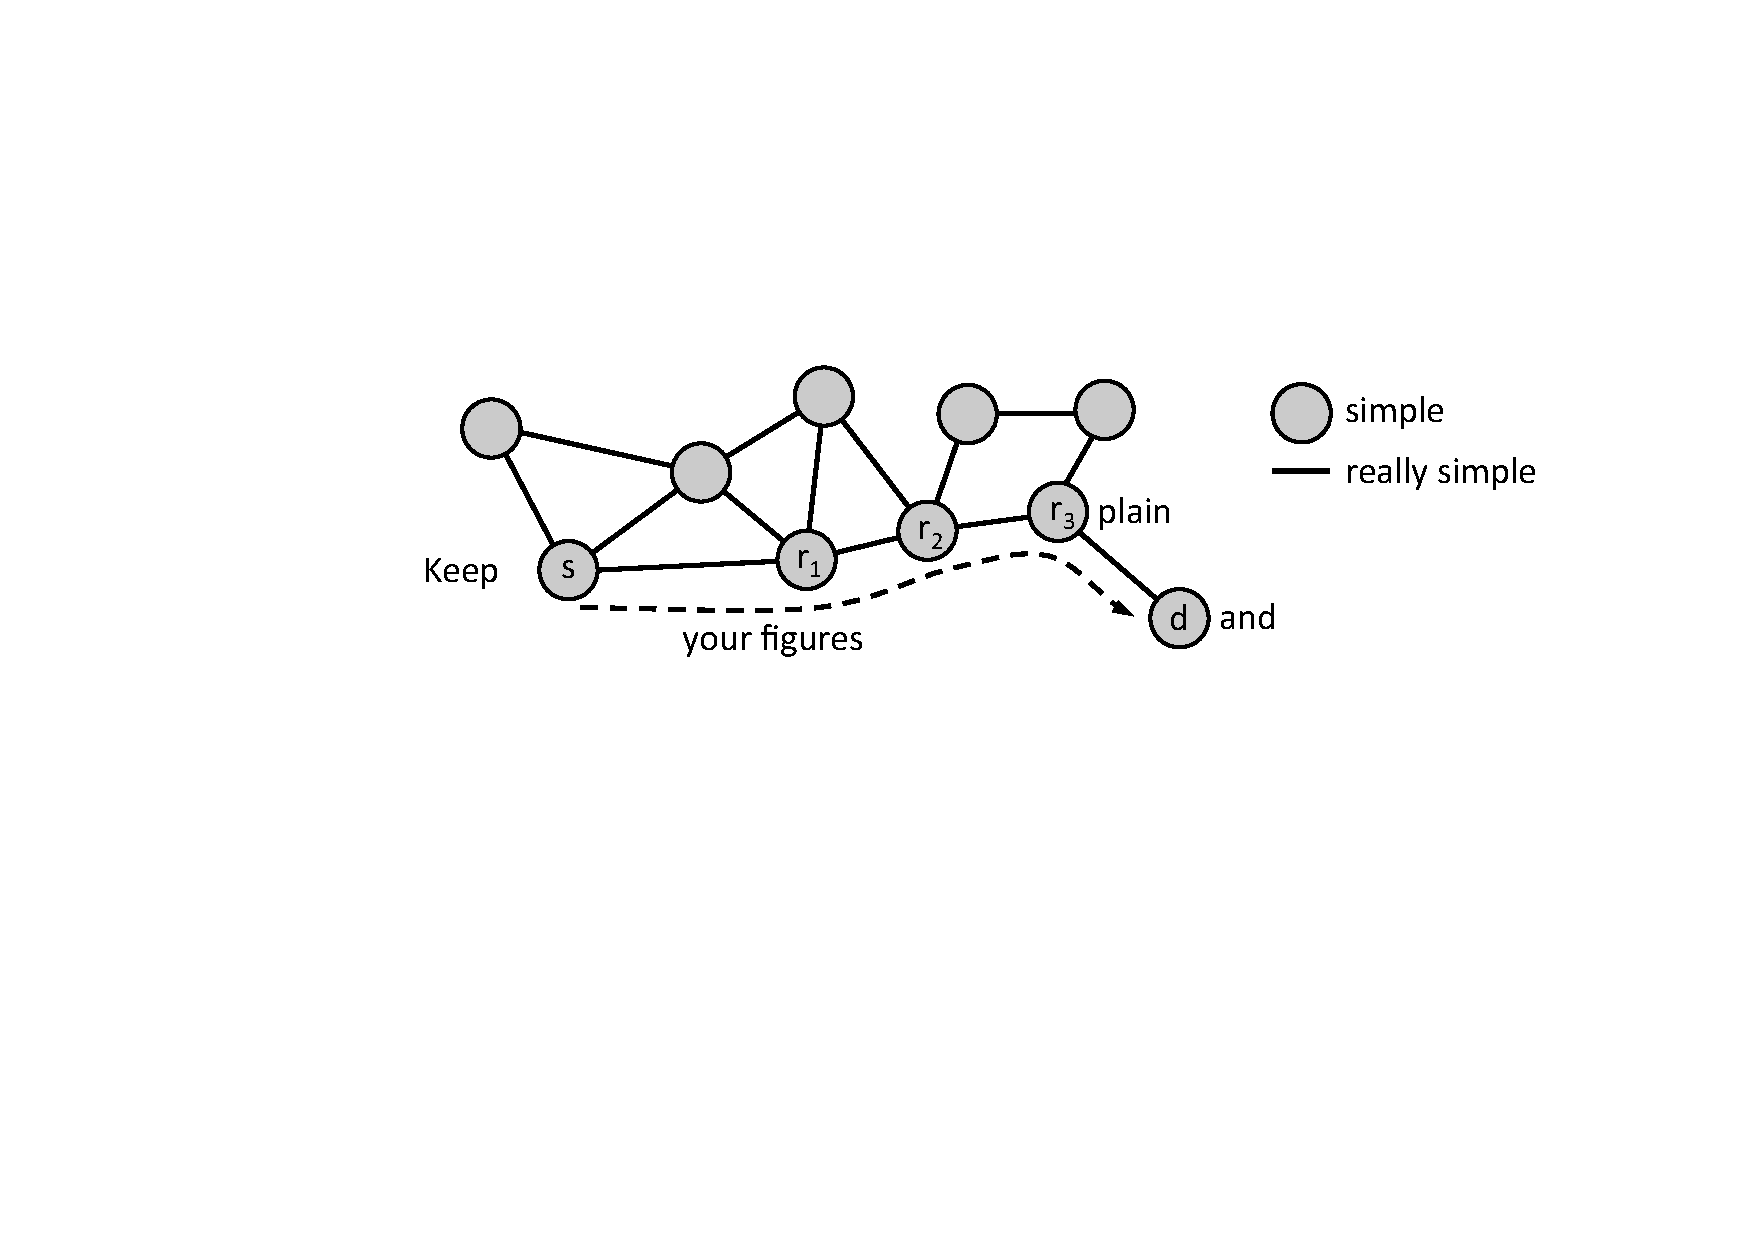
\includegraphics[width=1\columnwidth]{figures/example}
\caption{An example of an awesome image!}
\label{fig:example}
\end{figure}


Maecenas non tortor lorem, ac cursus nulla. Ut accumsan, felis vitae sollicitudin imperdiet, magna magna semper neque, faucibus feugiat augue neque vel risus. Quisque suscipit pellentesque felis, quis commodo felis mattis et. Maecenas ac augue sed enim posuere facilisis. Nam fringilla faucibus blandit. Morbi ante nisi, sodales in laoreet eu, fermentum sit amet tellus. Integer vel lorem turpis, eu commodo augue. Etiam vel tellus velit, et hendrerit magna. Nulla vitae tellus ut odio pellentesque varius eu eget turpis. In eros neque, rhoncus ac imperdiet eu, luctus eget mi.

Nulla sed lectus pulvinar tellus pretium dignissim pretium in dolor. Sed mollis ornare nisi. Nulla facilisi. Sed porta venenatis ultrices. Sed ut libero nec arcu lobortis suscipit non eget lacus. Donec egestas lacinia ligula, quis tristique eros dapibus eget. Suspendisse iaculis felis id lacus vestibulum malesuada. In vel tincidunt dui. In sed sapien nulla, sit amet venenatis felis. Integer quis leo ipsum, ac sagittis nibh. Curabitur interdum, turpis eu tincidunt ornare, arcu justo aliquet est, ut congue tortor dolor eget leo. Morbi viverra iaculis porttitor. Maecenas eleifend varius tellus, id ultricies sem dapibus id. Fusce lacinia arcu ac odio varius ac ultricies erat mollis. Lorem ipsum dolor sit amet, consectetur adipiscing elit.

\begin{description}
\item[Ut ac ipsum:]
Ut ac ipsum at velit malesuada tincidunt ornare at sapien. Aenean at dui dolor. Pellentesque sit amet fermentum lorem. Nullam pulvinar diam eget diam hendrerit condimentum. Duis fermentum vulputate ante, a egestas mauris vehicula at. Quisque convallis vestibulum fermentum.

\item[Aenean lacinia elementum:]
Aliquam sed ante id velit ultricies condimentum. Aenean lacinia elementum lacus sit amet luctus. Vestibulum consequat nibh et tortor laoreet sit amet vehicula orci venenatis. Suspendisse enim velit, hendrerit quis vestibulum sit amet, tincidunt sit amet odio.

\item[Phasellus id:]
Nullam ut est lacinia est auctor consectetur faucibus nec tellus. Phasellus id tincidunt risus. Nulla volutpat quam vel diam vehicula in egestas ligula laoreet.

\end{description}

In consequat laoreet blandit. Ut ac ipsum at velit malesuada tincidunt ornare at sapien. Aenean at dui dolor. Pellentesque sit amet fermentum lorem. Nullam pulvinar diam eget diam hendrerit condimentum. Duis fermentum vulputate ante, a egestas mauris vehicula at. Quisque convallis vestibulum fermentum. Aenean molestie dictum libero, a tincidunt lectus vestibulum in. Vivamus consequat purus pellentesque urna elementum consequat. Cras nec tortor felis, ac cursus risus. Morbi gravida ligula nec orci aliquam aliquam. Morbi et ligula diam, vel venenatis eros. Duis rhoncus ultricies mollis. Nullam ut est lacinia est auctor consectetur faucibus nec tellus. Phasellus id tincidunt risus. Nulla volutpat quam vel diam vehicula in egestas ligula laoreet.

\begin{table}[b]
\caption{Tables should look like this (save for the last row). If you know LaTeX better than me, feel free to improve the way of producing these tables.}
\begin{tabularx}{\linewidth}{|l|X|X|}
\hline
\rowcolor{slightgray}
\T Tables	&have gray  &headlines\\
\hline
\cellcolor{slightgray}\T and gray &labels \B&, too.\\
\hline
\cellcolor{slightgray}\T T &and B& are used for spacing\B\\
\hline
\cellcolor{slightgray} without T & and B& the cells are too small\B\\
\hline 
\end{tabularx}
\label{tab:example}
\end{table}

Lorem ipsum dolor sit amet, consectetur adipiscing elit. Vestibulum posuere vehicula lorem id commodo. Nam tempor felis quis orci tincidunt suscipit. Morbi dictum purus et nisl porttitor fringilla. Quisque feugiat, tellus quis semper placerat, lectus eros rutrum ipsum, eu elementum nibh nulla eu purus. Vestibulum ultrices varius orci, vitae porta elit laoreet at. Phasellus luctus aliquam molestie. Praesent varius blandit felis eu pellentesque. Aliquam erat volutpat. Morbi at est nibh.

Sed a mi tellus, id pellentesque neque. Integer vel volutpat diam. Sed nec lorem eu arcu lobortis porta. Sed quam nunc, luctus quis facilisis nec, aliquet nec mauris. Mauris non velit nisi, sed convallis risus. Sed quis lectus ligula. Morbi in nibh elit. Aenean a purus justo. Suspendisse pretium semper faucibus. Proin dictum, justo quis sagittis cursus, erat massa sollicitudin magna, in tempus quam lacus non turpis.

Cum sociis natoque penatibus et magnis dis parturient montes, nascetur ridiculus mus. Etiam congue magna at est pellentesque nec hendrerit arcu aliquet. Vivamus sem lectus, vehicula elementum accumsan iaculis, condimentum a mi. Proin sit amet justo eleifend massa eleifend lacinia. Mauris nibh nisl, vehicula vel tincidunt ac, varius et odio. Aliquam feugiat nulla ac felis interdum sodales. Etiam mollis arcu et mi scelerisque quis viverra est vestibulum. Mauris at massa libero, sit amet tincidunt elit. Mauris tempor lorem ut purus hendrerit non viverra nisi vehicula.

Vivamus ligula dui, semper sed consequat non, tempor ut diam. Morbi metus nisl, adipiscing feugiat malesuada viverra, blandit id nunc. Aliquam sed ante id velit ultricies condimentum. Aenean lacinia elementum lacus sit amet luctus. Vestibulum consequat nibh et tortor laoreet sit amet vehicula orci venenatis. Suspendisse enim velit, hendrerit quis vestibulum sit amet, tincidunt sit amet odio. Sed gravida tellus in nunc egestas porta. Morbi suscipit, dui vel elementum volutpat, lectus nulla elementum lacus, vitae dictum erat turpis ut ligula. Donec sit amet dolor ut urna vestibulum consequat nec et purus. In adipiscing lacus vel tellus fermentum quis cursus sapien egestas. Curabitur id ipsum erat. In lacinia adipiscing sapien at varius.

In consequat laoreet blandit. Ut ac ipsum at velit malesuada tincidunt ornare at sapien. Aenean at dui dolor. Pellentesque sit amet fermentum lorem. Nullam pulvinar diam eget diam hendrerit condimentum. Duis fermentum vulputate ante, a egestas mauris vehicula at. Quisque convallis vestibulum fermentum. Aenean molestie dictum libero, a tincidunt lectus vestibulum in. Vivamus consequat purus pellentesque urna elementum consequat. Cras nec tortor felis, ac cursus risus. Morbi gravida ligula nec orci aliquam aliquam. Morbi et ligula diam, vel venenatis eros. Duis rhoncus ultricies mollis. Nullam ut est lacinia est auctor consectetur faucibus nec tellus. Phasellus id tincidunt risus. Nulla volutpat quam vel diam vehicula in egestas ligula laoreet.

Maecenas non tortor lorem, ac cursus nulla. Ut accumsan, felis vitae sollicitudin imperdiet, magna magna semper neque, faucibus feugiat augue neque vel risus. Quisque suscipit pellentesque felis, quis commodo felis mattis et. Maecenas ac augue sed enim posuere facilisis. Nam fringilla faucibus blandit. Morbi ante nisi, sodales in laoreet eu, fermentum sit amet tellus. Integer vel lorem turpis, eu commodo augue. Etiam vel tellus velit, et hendrerit magna. Nulla vitae tellus ut odio pellentesque varius eu eget turpis. In eros neque, rhoncus ac imperdiet eu, luctus eget mi.

Nulla sed lectus pulvinar tellus pretium dignissim pretium in dolor. Sed mollis ornare nisi. Nulla facilisi. Sed porta venenatis ultrices. Sed ut libero nec arcu lobortis suscipit non eget lacus. Donec egestas lacinia ligula, quis tristique eros dapibus eget. Suspendisse iaculis felis id lacus vestibulum malesuada. In vel tincidunt dui. In sed sapien nulla, sit amet venenatis felis. Integer quis leo ipsum, ac sagittis nibh. Curabitur interdum, turpis eu tincidunt ornare, arcu justo aliquet est, ut congue tortor dolor eget leo. Morbi viverra iaculis porttitor. Maecenas eleifend varius tellus, id ultricies sem dapibus id. Fusce lacinia arcu ac odio varius ac ultricies erat mollis. Lorem ipsum dolor sit amet, consectetur adipiscing elit.

These are reference and cite examples. See \cref{fig:example}, \cref{tab:example}, and \cref{lst:example}. Cite early and often~\cite{exampleentry} is a good rule of thumb.


%%%%%%%%%%%%%%%%%%%%%%%%%%%%%%%%%%%%%%%%%%%%%%%%%%%%%%%%%%%%%
%% LITERATUR UND ANDERE VERZEICHNISSE
%%%%%%%%%%%%%%%%%%%%%%%%%%%%%%%%%%%%%%%%%%%%%%%%%%%%%%%%%%%%%
%% Ein kleiner Abstand zu den Kapiteln im Inhaltsverzeichnis (toc)
\ifnotdraft{
\addtocontents{toc}{\protect\vspace*{\baselineskip}}
\cleardoublepage
%% Literaturverzeichnis
\phantomsection % phantomsection wird benötigt, damit z.B. hyperref die richtige Seite verlinkt.
\addcontentsline{toc}{chapter}{Bibliography}
\begin{footnotesize}
%\nocite{*} %Auch nicht-zitierte BibTeX-Einträge werden angezeigt.
\bibliography{literature/literature}%Eine Datei 'literature.bib' wird hierfür benötigt.
\bibliographystyle{styles/comsys-alpha}%Art der Ausgabe: plain / apalike / amsalpha / ...
\end{footnotesize}
}

%% Abbildungsverzeichnis
%\clearpage
%\addcontentsline{toc}{chapter}{List of Figures}
%\listoffigures

%% Tabellenverzeichnis
%\clearpage
%\addcontentsline{toc}{chapter}{List of Tables}
%\listoftables


%%%%%%%%%%%%%%%%%%%%%%%%%%%%%%%%%%%%%%%%%%%%%%%%%%%%%%%%%%%%%
%% ANHÄNGE
%%%%%%%%%%%%%%%%%%%%%%%%%%%%%%%%%%%%%%%%%%%%%%%%%%%%%%%%%%%%%
\appendix
% !TEX root = ../thesis.tex

\chapter{Appendix}

\printacronyms[heading=section,name=List of Abbreviations]{}



\end{document}
